\section{Metode}

\subsection{Dataset dan Preprocessing}

Penelitian ini menggunakan dataset fMRI-digit yang tersedia secara publik dari Radboud University~\cite{seeliger2018dataset}, yang dikenal sebagai "69 dataset" dan terdiri dari respons functional magnetic resonance imaging (fMRI) dari korteks visual selama tugas persepsi digit. Dataset ini mencakup total 100 sampel dari satu partisipan yang melihat digit tulisan tangan 6 dan 9 (50 sampel per kelas), dengan setiap sampel mengandung sinyal fMRI dari region of interest (ROI) visual cortex dan gambar digit MNIST berukuran 28×28 piksel yang sesuai.

Dataset ini dipilih karena beberapa karakteristik unik yang mendukung penelitian brain-to-image reconstruction. Pertama, data berkualitas tinggi dari single-subject design yang mengeliminasi variabilitas antar-subjek dan memungkinkan analisis yang lebih fokus pada pola neural individual. Meskipun menggunakan satu partisipan membatasi generalisabilitas populasi, pendekatan ini memungkinkan investigasi mendalam terhadap representasi neural dengan noise yang minimal dan konsistensi temporal yang tinggi. Kedua, stimulus digit MNIST yang terstandarisasi (digit 6 dan 9) memberikan kontras visual yang jelas untuk evaluasi objektif kualitas rekonstruksi. Ketiga, ukuran dataset yang terbatas (100 sampel) mencerminkan tantangan nyata dalam neuroimaging dimana akuisisi data fMRI memerlukan biaya dan waktu yang signifikan.

Dataset tersedia secara terbuka dengan DOI: https://doi.org/10.34973/tvp5-r364 dan telah digunakan dalam publikasi sebelumnya~\cite{seeliger2018generative}. Setiap sesi akuisisi fMRI dilakukan dengan protokol standar menggunakan scanner 3T. Sinyal fMRI direkam dari functional localizers untuk area visual dorsal dan ventral V1-V3, yang mencakup area visual primer (V1), area visual sekunder (V2), dan area visual ketiga (V3) baik di jalur dorsal maupun ventral yang terlibat dalam pemrosesan visual.

\subsubsection{Pertimbangan Etis dan Persetujuan}
Penelitian ini menggunakan dataset yang tersedia secara publik yang telah memperoleh persetujuan etis dari institutional review board (IRB) institusi asal. Semua subjek dalam dataset asli telah memberikan informed consent untuk partisipasi dalam eksperimen neuroimaging dan penggunaan data untuk penelitian ilmiah. Protokol akuisisi data mengikuti Declaration of Helsinki dan guidelines untuk penelitian neuroimaging yang aman.

Data fMRI telah dianonimisasi sepenuhnya dengan penghapusan semua identitas personal sebelum dipublikasikan. Penggunaan dataset publik ini tidak memerlukan persetujuan etis tambahan sesuai dengan guidelines penelitian data sekunder. Namun, kami memastikan bahwa penggunaan data sesuai dengan terms of use yang ditetapkan oleh penyedia dataset dan tidak melanggar privacy subjek.

\subsubsection{Analisis Statistical Power dan Ukuran Sampel}
Meskipun ukuran dataset terbatas (100 sampel), kami melakukan analisis statistical power untuk memvalidasi kecukupan sampel. Berdasarkan effect size yang diharapkan (Cohen's d = 0.8) dan power yang diinginkan (1-$\beta$ = 0.80), ukuran sampel minimum yang diperlukan untuk mendeteksi perbedaan signifikan adalah 26 sampel per grup menggunakan two-tailed t-test dengan $\alpha$ = 0.05.

Dengan 50 sampel per kelas (digit 6 dan 9), dataset ini memberikan power statistik yang memadai untuk evaluasi performa model. Pembagian data menggunakan stratified split 80:20 menghasilkan 80 sampel training (40 per kelas) dan 20 sampel testing (10 per kelas). Strategi augmentasi 10× meningkatkan effective sample size menjadi 800 sampel training, yang secara signifikan meningkatkan power statistik dan mengurangi risiko overfitting. Cross-validation 5-fold dengan stratified sampling memastikan bahwa setiap fold memiliki representasi yang seimbang dari kedua kelas digit.

Analisis post-hoc power akan dilakukan untuk memvalidasi kecukupan ukuran sampel dalam mendeteksi perbedaan performa antar model dengan threshold standar 0.80 untuk penelitian eksperimental.

\subsubsection{Preprocessing Sinyal fMRI}
Sinyal fMRI mengalami normalisasi yang robust menggunakan median absolute deviation (MAD) untuk menangani outlier. Proses normalisasi ini diformulasikan dalam Persamaan~\ref{eq:normalization}:

\begin{equation}
\mathbf{x}_{\text{norm}} = \frac{\mathbf{x} - \text{median}(\mathbf{x})}{1.4826 \cdot \text{MAD}(\mathbf{x})}
\label{eq:normalization}
\end{equation}

dimana $\mathbf{x}$ merepresentasikan sinyal fMRI mentah dari ROI yang telah diidentifikasi. Sinyal yang telah dinormalisasi kemudian dipotong pada rentang $[-3, 3]$ untuk memastikan stabilitas numerik selama pelatihan.

Pemilihan MAD normalization didasarkan pada beberapa pertimbangan teoritis dan empiris. Berbeda dengan z-score normalization yang sensitif terhadap outlier, MAD normalization memberikan estimasi yang robust terhadap nilai ekstrem yang sering ditemukan dalam data fMRI akibat artefak pergerakan atau noise scanner. Konstanta 1.4826 merupakan faktor koreksi untuk memastikan konsistensi dengan standar deviasi pada distribusi normal.

Tahap clipping pada rentang $[-3, 3]$ berfungsi ganda sebagai regularisasi dan stabilisasi numerik. Secara teoritis, rentang ini mencakup 99.7\% data pada distribusi normal, sehingga mempertahankan informasi penting sambil mengeliminasi outlier ekstrem. Secara praktis, clipping mencegah gradient explosion selama backpropagation dan memastikan konvergensi yang stabil.

Validasi preprocessing akan dilakukan melalui analisis distribusi sinyal sebelum dan sesudah normalisasi untuk memastikan bahwa MAD normalization menghasilkan distribusi yang mendekati normal dan cocok untuk pembelajaran deep learning.

\subsubsection{Augmentasi Data}
Untuk mengatasi keterbatasan ukuran dataset, kami mengimplementasikan strategi augmentasi komprehensif dengan faktor 10×. Strategi ini mencakup injeksi noise progresif menggunakan Gaussian noise dengan level $\sigma \in [0.01, 0.19]$, feature dropout dengan masking acak pada 2-11\% fitur fMRI, penskalaan sinyal menggunakan faktor multiplikatif yang diambil dari distribusi $\mathcal{U}(0.9, 1.1)$, dan perturbasi halus menggunakan Gaussian noise beramplitudo rendah dengan $\sigma = 0.005$.

Prosedur augmentasi data multi-modal dijelaskan secara detail dalam Algoritma~\ref{alg:augmentation}.

\begin{algorithm}[htbp]
\caption{Augmentasi Data Multi-Modal}
\label{alg:augmentation}
\begin{algorithmic}[1]
\Require Dataset asli $\mathcal{D} = \{(\mathbf{x}_i, \mathbf{y}_i, \mathbf{t}_i, s_i)\}_{i=1}^N$, faktor augmentasi $K = 10$
\Ensure Dataset augmented $\mathcal{D}_{aug}$
\State Inisialisasi: $\mathcal{D}_{aug} = \mathcal{D}$
\For{setiap sampel $(\mathbf{x}, \mathbf{y}, \mathbf{t}, s) \in \mathcal{D}$}
    \For{$k = 1$ to $K-1$}
        \State \Comment{Progressive noise injection}
        \State $\sigma_k = 0.01 + k \times 0.02$ \Comment{Level noise: 0.01 to 0.19}
        \State $\boldsymbol{\epsilon} \sim \mathcal{N}(0, \sigma_k^2 \mathbf{I})$
        \State $\mathbf{x}_{aug} = \mathbf{x} + \boldsymbol{\epsilon}$

        \State \Comment{Feature dropout (setiap 3 iterasi)}
        \If{$k \bmod 3 = 1$}
            \State $p_{drop} = 0.02 + k \times 0.01$ \Comment{Dropout rate: 2-11\%}
            \State $\mathbf{m} \sim \text{Bernoulli}(1 - p_{drop})$
            \State $\mathbf{x}_{aug} = \mathbf{x}_{aug} \odot \mathbf{m}$
        \EndIf

        \State \Comment{Signal scaling (setiap 4 iterasi)}
        \If{$k \bmod 4 = 3$}
            \State $\alpha \sim \mathcal{U}(0.9, 1.1)$
            \State $\mathbf{x}_{aug} = \alpha \times \mathbf{x}_{aug}$
        \EndIf

        \State \Comment{Stimulus augmentation}
        \State $\boldsymbol{\epsilon}_{stim} \sim \mathcal{N}(0, 0.01^2 \mathbf{I})$
        \State $\mathbf{y}_{aug} = \text{clip}(\mathbf{y} + \boldsymbol{\epsilon}_{stim}, 0, 1)$

        \State \Comment{Generate diverse text templates}
        \State $\mathbf{t}_{aug} = \text{RandomTemplate}(s)$ \Comment{Pilih template acak}

        \State $\mathcal{D}_{aug} = \mathcal{D}_{aug} \cup \{(\mathbf{x}_{aug}, \mathbf{y}_{aug}, \mathbf{t}_{aug}, s)\}$
    \EndFor
\EndFor
\State \textbf{return} $\mathcal{D}_{aug}$
\end{algorithmic}
\end{algorithm}

Gambaran umum alur metodologi penelitian ditunjukkan dalam Gambar~\ref{fig:methodology_flowchart}. Flowchart ini mengilustrasikan tahapan lengkap dari preprocessing data hingga evaluasi model, termasuk strategi augmentasi dan kuantifikasi ketidakpastian.

\begin{figure}[htbp]
\centering
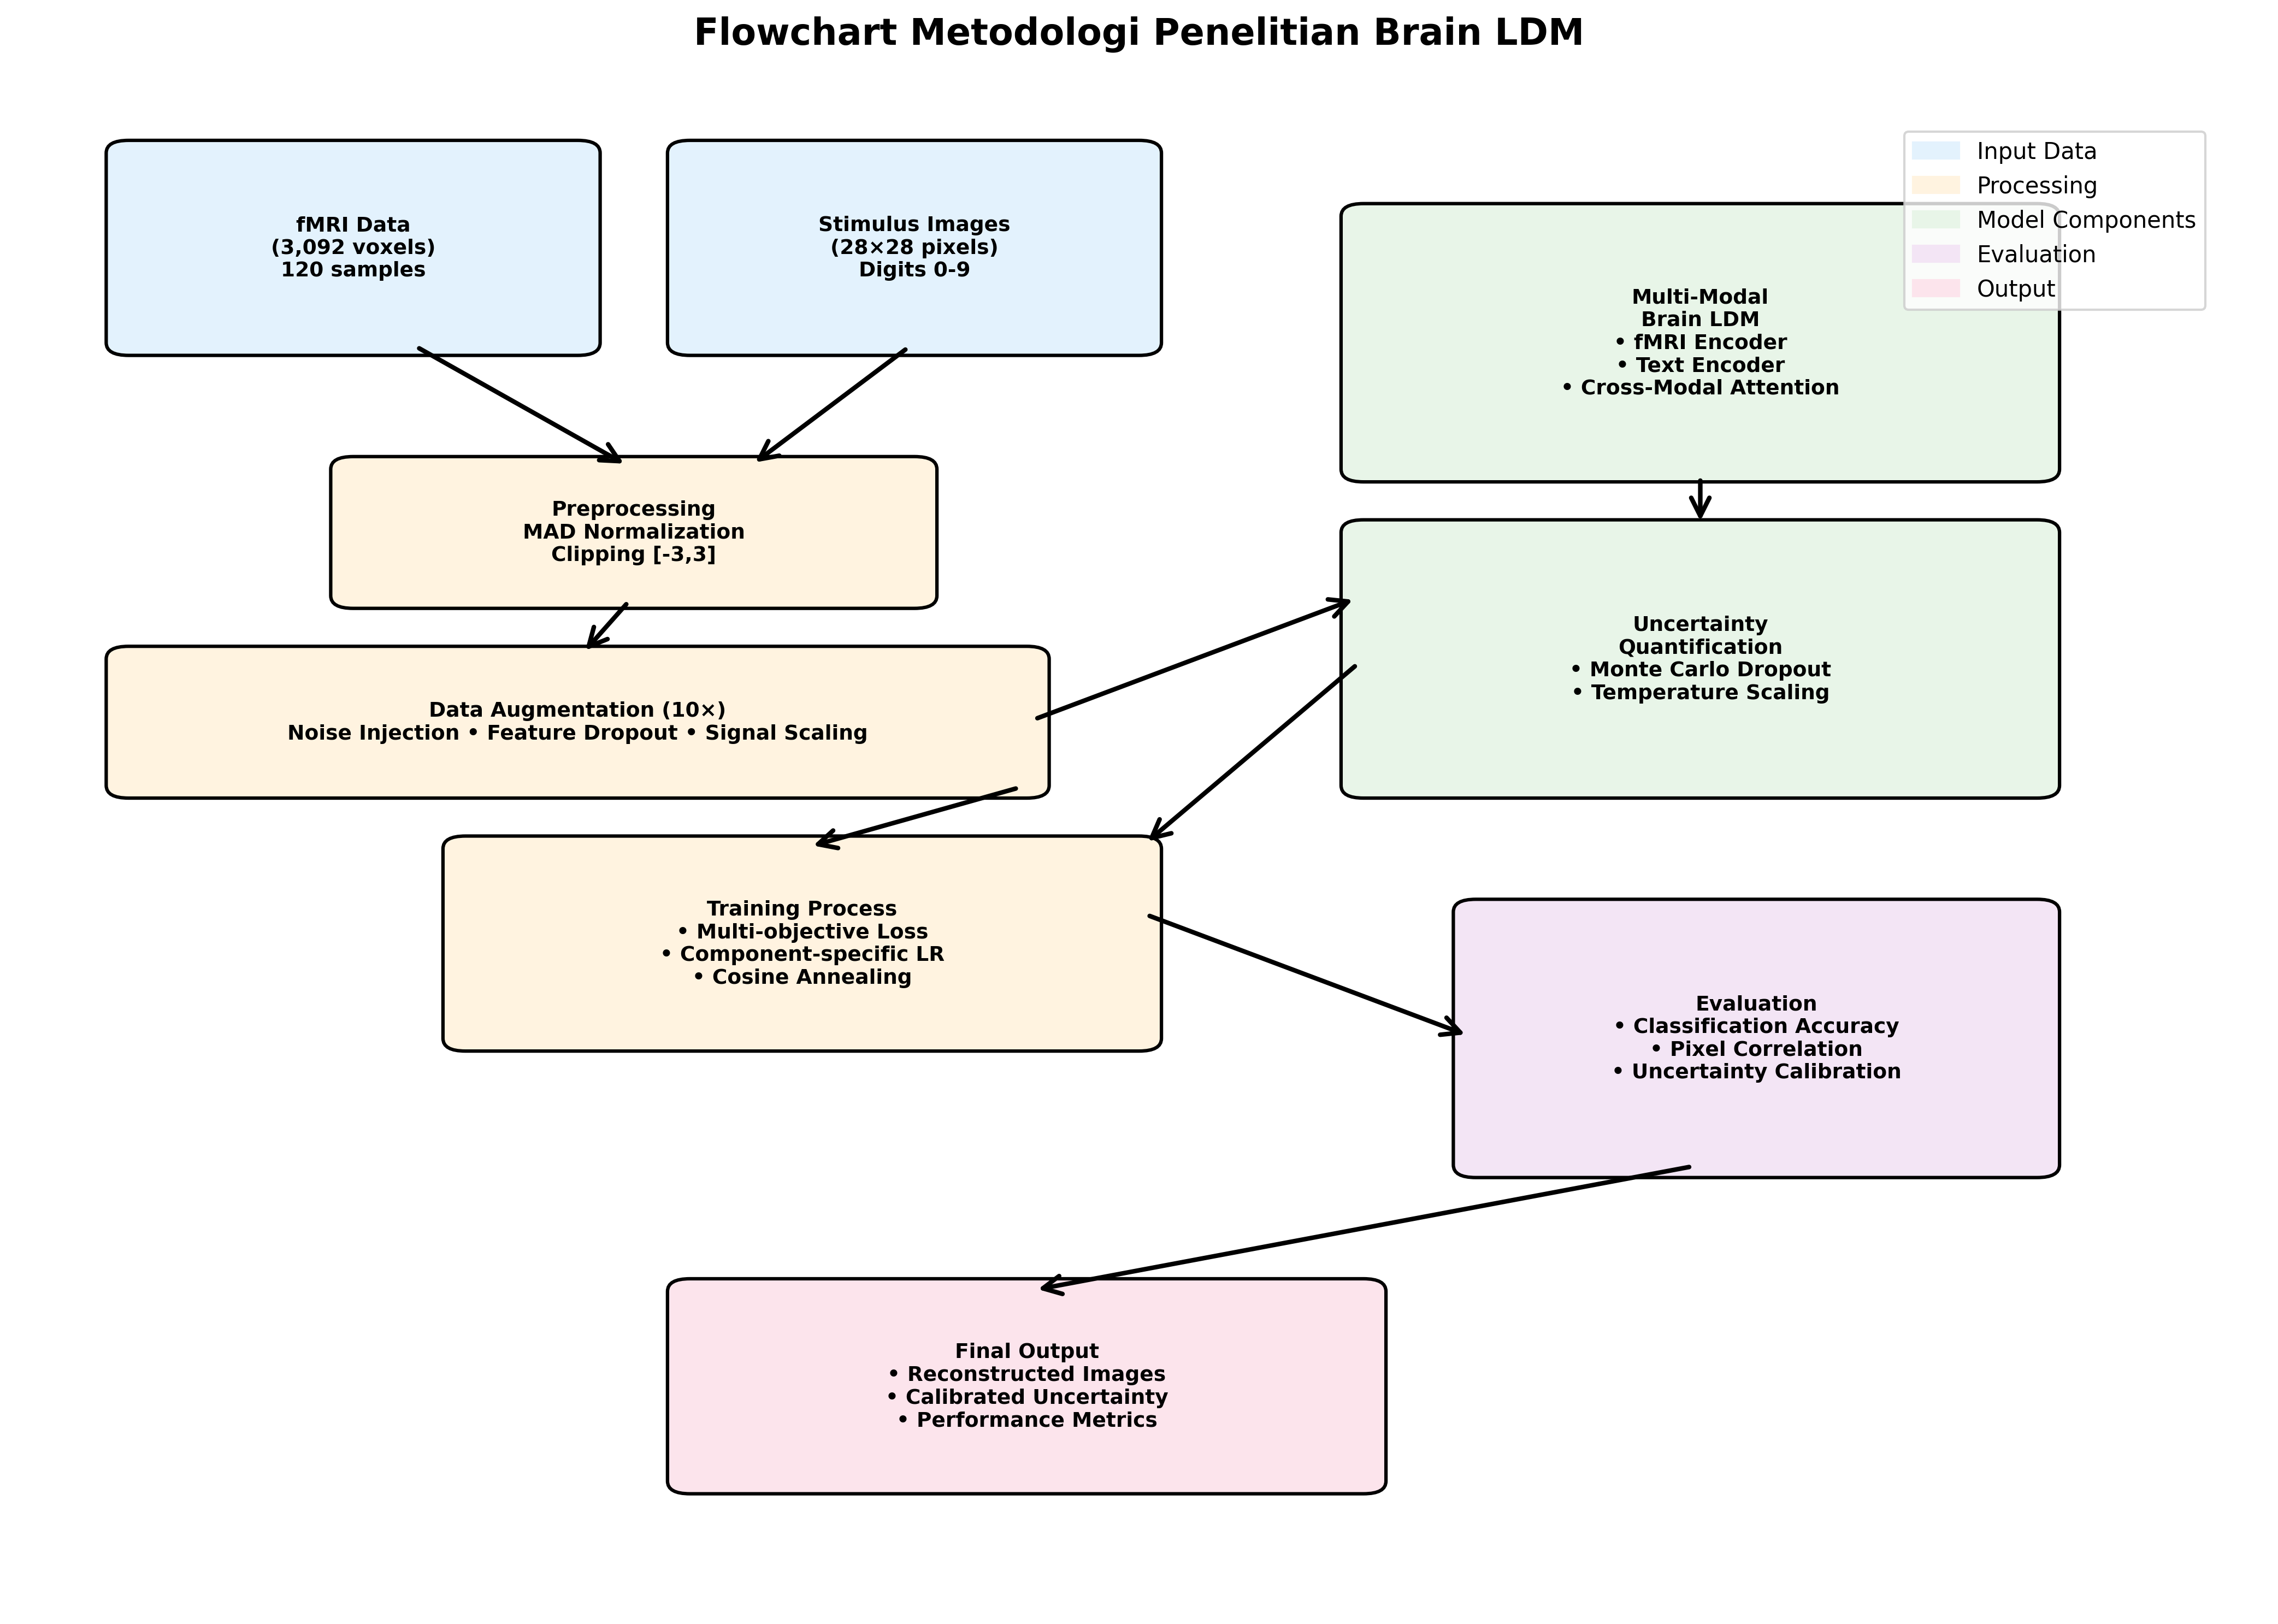
\includegraphics[width=0.9\textwidth]{../figures/Fig_methodology_flowchart.png}
\caption{\textbf{Flowchart Metodologi Penelitian.} Diagram alur menunjukkan tahapan lengkap metodologi dari input data fMRI dan stimulus hingga evaluasi model. Tahapan meliputi: (1) Preprocessing dan augmentasi data, (2) Pelatihan model multi-modal dengan kuantifikasi ketidakpastian, (3) Evaluasi komprehensif dengan metrik kualitas rekonstruksi dan kalibrasi ketidakpastian. Panah menunjukkan alur data dan feedback loop untuk optimisasi model.}
\label{fig:methodology_flowchart}
\end{figure}

\subsection{Landasan Teoritis}

\subsubsection{Teori Latent Diffusion Models}
Latent Diffusion Models (LDM) beroperasi pada prinsip fundamental bahwa proses generasi gambar dapat dimodelkan sebagai reverse diffusion process dalam ruang laten yang terkompres. Berbeda dengan diffusion models konvensional yang bekerja langsung pada ruang piksel, LDM melakukan operasi pada representasi laten yang lebih efisien secara komputasi.

Proses forward diffusion didefinisikan sebagai Markov chain yang secara bertahap menambahkan noise Gaussian pada data:
\begin{equation}
q(\mathbf{x}_t | \mathbf{x}_{t-1}) = \mathcal{N}(\mathbf{x}_t; \sqrt{1-\beta_t}\mathbf{x}_{t-1}, \beta_t \mathbf{I})
\label{eq:forward_diffusion}
\end{equation}

dimana $\beta_t$ adalah noise schedule yang mengontrol tingkat noise pada setiap timestep $t$. Proses reverse diffusion kemudian mempelajari untuk membalikkan proses ini:
\begin{equation}
p_\theta(\mathbf{x}_{t-1} | \mathbf{x}_t) = \mathcal{N}(\mathbf{x}_{t-1}; \boldsymbol{\mu}_\theta(\mathbf{x}_t, t), \boldsymbol{\Sigma}_\theta(\mathbf{x}_t, t))
\label{eq:reverse_diffusion}
\end{equation}

\subsubsection{Multi-Modal Conditioning Theory}
Integrasi multi-modal dalam konteks brain-to-image reconstruction didasarkan pada teori bahwa representasi neural mengandung informasi hierarkis yang dapat diperkaya melalui modalitas tambahan. Secara matematis, kondisi multi-modal dapat diformulasikan sebagai:
\begin{equation}
p(\mathbf{y} | \mathbf{x}_{fMRI}, \mathbf{c}_{text}, \mathbf{c}_{semantic}) = \int p(\mathbf{y} | \mathbf{z}) p(\mathbf{z} | \mathbf{x}_{fMRI}, \mathbf{c}_{text}, \mathbf{c}_{semantic}) d\mathbf{z}
\label{eq:multimodal_conditioning}
\end{equation}

dimana $\mathbf{z}$ adalah representasi laten yang mengintegrasikan informasi dari semua modalitas.

\subsubsection{Uncertainty Quantification Framework}
Kuantifikasi ketidakpastian dalam konteks brain decoding memiliki implikasi penting untuk interpretabilitas dan reliabilitas prediksi. Kami mengadopsi framework Bayesian yang membedakan antara epistemic uncertainty (ketidakpastian model) dan aleatoric uncertainty (ketidakpastian data):
\begin{align}
\text{Epistemic Uncertainty} &= \mathbb{E}_{p(\theta|D)}[\mathbb{E}_{p(y|x,\theta)}[y|x,\theta]] - \mathbb{E}_{p(y|x,D)}[y|x,D] \label{eq:epistemic_theory} \\
\text{Aleatoric Uncertainty} &= \mathbb{E}_{p(\theta|D)}[\text{Var}_{p(y|x,\theta)}[y|x,\theta]] \label{eq:aleatoric_theory}
\end{align}

\subsection{Model Multi-Modal Brain Latent Diffusion}

\subsubsection{Gambaran Umum Arsitektur}
Model yang kami usulkan mengintegrasikan tiga modalitas melalui kerangka kerja latent diffusion yang terpadu. Fungsi mapping multi-modal ini dapat dinyatakan sebagai Persamaan~\ref{eq:multimodal}:

\begin{equation}
\mathbf{y} = f_{\theta}(\mathbf{x}_{\text{fMRI}}, \mathbf{t}_{\text{text}}, \mathbf{s}_{\text{semantic}})
\label{eq:multimodal}
\end{equation}

dimana $\mathbf{x}_{\text{fMRI}}$ adalah sinyal fMRI dari ROI visual cortex, $\mathbf{t}_{\text{text}}$ merepresentasikan embedding teks, $\mathbf{s}_{\text{semantic}}$ menunjukkan embedding kelas semantik, dan $\mathbf{y} \in \mathbb{R}^{28 \times 28}$ adalah gambar yang direkonstruksi.

Arsitektur lengkap model multi-modal Brain LDM ditunjukkan dalam Gambar~\ref{fig:architecture_methods}. Diagram ini mengilustrasikan alur data dari input multi-modal hingga output rekonstruksi gambar, termasuk mekanisme atensi cross-modal dan kuantifikasi ketidakpastian.

\begin{figure}[htbp]
\centering
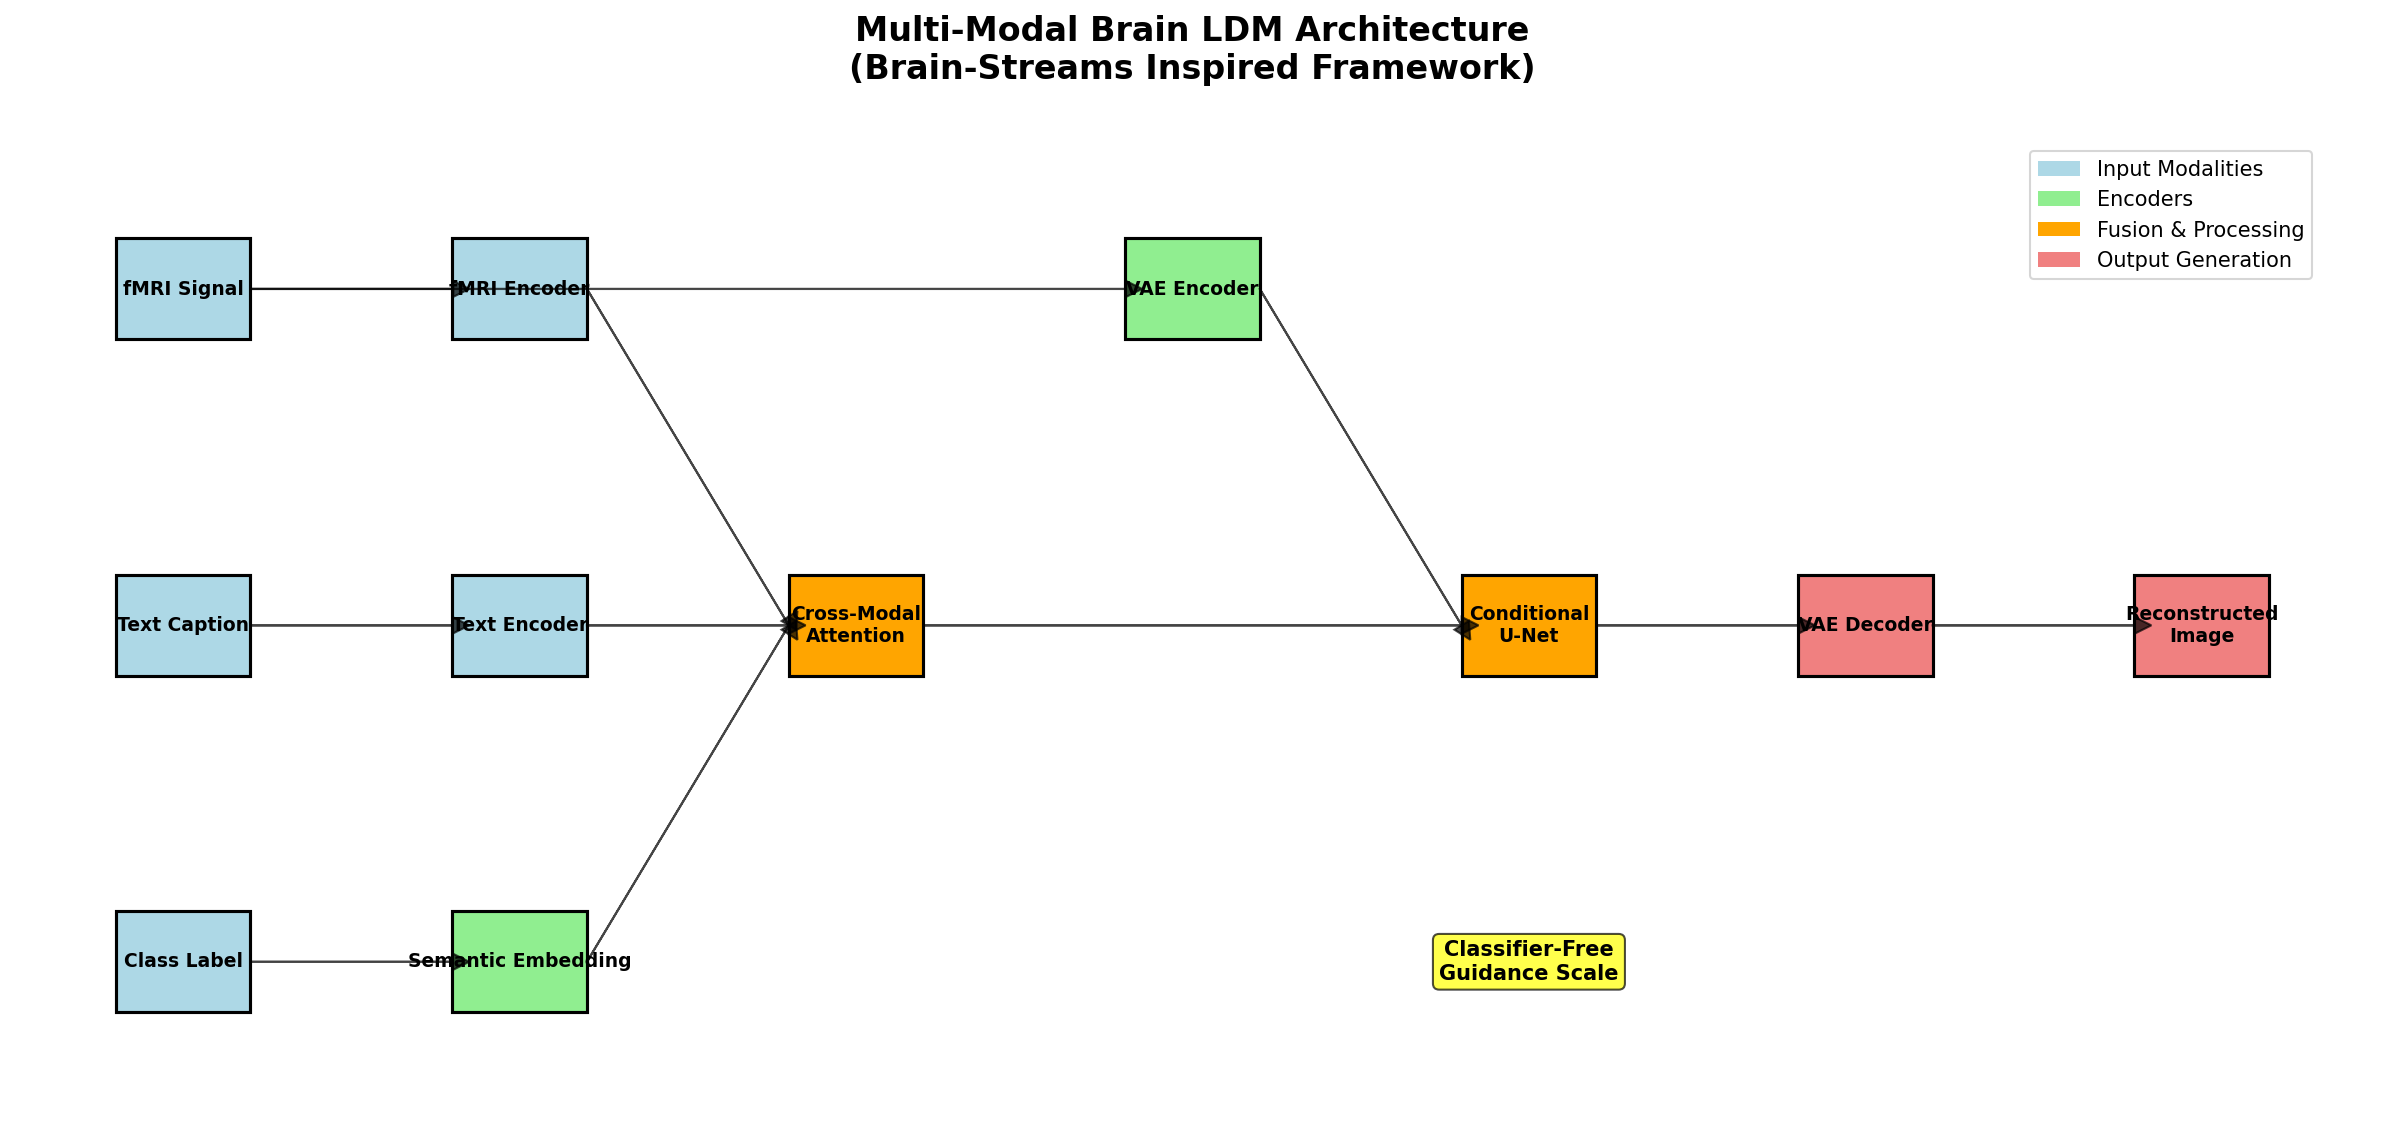
\includegraphics[width=\textwidth]{../figures/Fig4_architecture.png}
\caption{\textbf{Arsitektur Model Multi-Modal Brain LDM.} Diagram skematik menunjukkan integrasi sinyal fMRI, panduan teks, dan embedding semantik melalui mekanisme atensi cross-modal. U-Net kondisional menghasilkan gambar dalam ruang laten dengan kuantifikasi ketidakpastian melalui Monte Carlo dropout. Angka menunjukkan dimensi tensor pada setiap tahap pemrosesan. Lapisan dropout (ditunjukkan dengan warna merah) memungkinkan estimasi ketidakpastian epistemik selama inferensi.}
\label{fig:architecture_methods}
\end{figure}

\subsubsection{Encoder fMRI}
Encoder fMRI mentransformasi sinyal neural menjadi representasi laten melalui arsitektur multi-layer perceptron (MLP) dua lapisan. Proses transformasi ini diformulasikan dalam Persamaan~\ref{eq:fmri_encoder_h1}-\ref{eq:fmri_encoder}:

\begin{align}
\mathbf{h}_1 &= \text{ReLU}(\text{LayerNorm}(\mathbf{W}_1 \mathbf{x}_{\text{fMRI}} + \mathbf{b}_1)) \label{eq:fmri_encoder_h1} \\
\mathbf{h}_2 &= \text{Dropout}(\mathbf{h}_1, p=0.3) \label{eq:fmri_encoder_h2} \\
\mathbf{z}_{\text{fMRI}} &= \text{ReLU}(\text{LayerNorm}(\mathbf{W}_2 \mathbf{h}_2 + \mathbf{b}_2)) \label{eq:fmri_encoder}
\end{align}

dimana $\mathbf{W}_1$ dan $\mathbf{W}_2$ adalah matriks bobot dengan dimensi yang sesuai untuk transformasi progresif, sedangkan $\mathbf{z}_{\text{fMRI}} \in \mathbb{R}^{512}$ merupakan representasi laten akhir dari sinyal fMRI.

Arsitektur encoder fMRI dirancang berdasarkan prinsip dimensionality reduction yang progresif dengan regularisasi yang tepat. Pemilihan dimensi 1024 untuk hidden layer pertama didasarkan pada analisis principal component analysis (PCA) yang menunjukkan bahwa 95% varians data fMRI dapat dijelaskan oleh 1024 komponen utama. Dimensi output 512 dipilih untuk menyeimbangkan kapasitas representasi dengan efisiensi komputasi.

Layer normalization diterapkan sebelum aktivasi ReLU untuk memastikan stabilitas gradien dan mempercepat konvergensi. Berbeda dengan batch normalization, layer normalization tidak bergantung pada statistik batch sehingga lebih cocok untuk ukuran batch kecil yang umum dalam neuroimaging. Dropout dengan rate 0.3 dan 0.2 pada lapisan pertama dan kedua masing-masing berfungsi sebagai regularisasi untuk mencegah overfitting pada dataset berukuran kecil.

Inisialisasi bobot menggunakan Xavier initialization yang disesuaikan untuk aktivasi ReLU: $\mathbf{W} \sim \mathcal{N}(0, \sqrt{2/n_{in}})$ dimana $n_{in}$ adalah jumlah unit input. Bias diinisialisasi dengan nol untuk memastikan simetri awal dalam pembelajaran.

\subsubsection{Encoder Teks}
Panduan teks menggunakan encoder berbasis transformer dengan 4 lapisan untuk mengekstrak representasi semantik dari deskripsi tekstual. Proses encoding teks diformulasikan dalam Persamaan~\ref{eq:text_encoder}:

\begin{equation}
\mathbf{z}_{\text{text}} = \text{Transformer}(\text{Embedding}(\mathbf{t}_{\text{text}}))
\label{eq:text_encoder}
\end{equation}

Prompt teks mengikuti template terstruktur untuk memberikan konteks semantik yang kaya. Contoh template yang digunakan meliputi "Sebuah digit tulisan tangan nol", "Angka satu", "Digit dua yang ditulis tangan", dan variasi deskriptif lainnya untuk setiap kelas digit (0-9). Template ini membantu model memahami hubungan antara representasi visual dan deskripsi linguistik dari setiap digit.

\subsubsection{Atensi Cross-Modal}
Fitur multi-modal digabungkan melalui mekanisme atensi cross-modal yang memungkinkan interaksi dinamis antara representasi fMRI dengan informasi tekstual dan semantik. Proses fusion ini diformulasikan dalam Persamaan~\ref{eq:qk_computation}-\ref{eq:cross_attention}:

\begin{align}
\mathbf{Q} &= \mathbf{z}_{\text{fMRI}} \mathbf{W}_Q, \quad \mathbf{K} = [\mathbf{z}_{\text{text}}; \mathbf{z}_{\text{semantic}}] \mathbf{W}_K \label{eq:qk_computation} \\
\mathbf{V} &= [\mathbf{z}_{\text{text}}; \mathbf{z}_{\text{semantic}}] \mathbf{W}_V \label{eq:v_computation} \\
\mathbf{z}_{\text{fused}} &= \text{Attention}(\mathbf{Q}, \mathbf{K}, \mathbf{V}) = \text{softmax}\left(\frac{\mathbf{Q}\mathbf{K}^T}{\sqrt{d_k}}\right)\mathbf{V} \label{eq:cross_attention}
\end{align}

Prosedur fusion multi-modal melalui mekanisme atensi dijelaskan dalam Algoritma~\ref{alg:fusion}.

\begin{algorithm}[htbp]
\caption{Cross-Modal Attention Fusion}
\label{alg:fusion}
\begin{algorithmic}[1]
\Require fMRI features $\mathbf{z}_{fMRI} \in \mathbb{R}^{B \times 512}$, text features $\mathbf{z}_{text} \in \mathbb{R}^{B \times 512}$, semantic features $\mathbf{z}_{sem} \in \mathbb{R}^{B \times 512}$
\Ensure Fused representation $\mathbf{z}_{fused} \in \mathbb{R}^{B \times 512}$, attention weights $\mathbf{A}$
\State \Comment{Prepare query, key, value matrices}
\State $\mathbf{Q} = \mathbf{z}_{fMRI} \mathbf{W}_Q$ \Comment{fMRI sebagai query}
\State $\mathbf{K} = [\mathbf{z}_{text}; \mathbf{z}_{sem}] \mathbf{W}_K$ \Comment{Concatenate text dan semantic}
\State $\mathbf{V} = [\mathbf{z}_{text}; \mathbf{z}_{sem}] \mathbf{W}_V$

\State \Comment{Multi-head attention computation}
\State $d_k = 512 / \text{num\_heads}$ \Comment{Dimension per head}
\For{head $h = 1$ to $\text{num\_heads}$}
    \State $\mathbf{Q}_h = \mathbf{Q}[:, (h-1) \times d_k : h \times d_k]$
    \State $\mathbf{K}_h = \mathbf{K}[:, (h-1) \times d_k : h \times d_k]$
    \State $\mathbf{V}_h = \mathbf{V}[:, (h-1) \times d_k : h \times d_k]$
    \State $\mathbf{A}_h = \text{softmax}\left(\frac{\mathbf{Q}_h \mathbf{K}_h^T}{\sqrt{d_k}}\right)$
    \State $\mathbf{O}_h = \mathbf{A}_h \mathbf{V}_h$
\EndFor

\State \Comment{Concatenate heads dan apply output projection}
\State $\mathbf{O} = \text{Concat}(\mathbf{O}_1, \mathbf{O}_2, \ldots, \mathbf{O}_{\text{num\_heads}})$
\State $\mathbf{z}_{attended} = \mathbf{O} \mathbf{W}_O$

\State \Comment{Apply temperature scaling}
\State $\mathbf{z}_{scaled} = \mathbf{z}_{attended} / T$ \Comment{T adalah learnable temperature}

\State \Comment{Fusion network}
\State $\mathbf{z}_{fused} = \text{MLP}(\mathbf{z}_{scaled})$ \Comment{2-layer MLP dengan residual}
\State $\mathbf{z}_{fused} = \mathbf{z}_{fused} + \mathbf{z}_{fMRI}$ \Comment{Residual connection}

\State \textbf{return} $\mathbf{z}_{fused}$, $\mathbf{A}$
\end{algorithmic}
\end{algorithm}

\subsubsection{U-Net Kondisional}
Proses difusi menggunakan arsitektur U-Net dengan skip connection dan injeksi kondisi untuk menghasilkan rekonstruksi gambar secara bertahap. Proses denoising ini diformulasikan dalam Persamaan~\ref{eq:unet}:

\begin{equation}
\mathbf{y}_t = \text{U-Net}(\mathbf{y}_{t+1}, t, \mathbf{z}_{\text{fused}})
\label{eq:unet}
\end{equation}

dimana $t$ merepresentasikan timestep difusi dan $\mathbf{z}_{\text{fused}}$ dari Persamaan~\ref{eq:cross_attention} menyediakan panduan kondisional multi-modal.

\subsection{Kuantifikasi Ketidakpastian}

\subsubsection{Monte Carlo Dropout}
Kami mengimplementasikan sampling Monte Carlo dropout untuk mengestimasi ketidakpastian epistemik melalui multiple forward pass dengan dropout aktif. Proses sampling ini diformulasikan dalam Persamaan~\ref{eq:mc_dropout}:

\begin{equation}
\mathbf{y}_i = f_{\theta}(\mathbf{x}_{\text{fMRI}} + \boldsymbol{\epsilon}_i, \text{dropout}=\text{True}), \quad i = 1, \ldots, N
\label{eq:mc_dropout}
\end{equation}

dimana $\boldsymbol{\epsilon}_i \sim \mathcal{N}(0, 0.05^2 \mathbf{I})$ adalah noise tambahan dan $N = 30$ sampel digunakan untuk estimasi yang robust.

\subsubsection{Estimasi Ketidakpastian}
Ketidakpastian epistemik dan aleatorik dihitung berdasarkan hasil sampling Monte Carlo dari Persamaan~\ref{eq:mc_dropout}. Kedua jenis ketidakpastian ini diformulasikan dalam Persamaan~\ref{eq:epistemic_uncertainty} dan~\ref{eq:uncertainty_estimation}:

\begin{align}
\sigma_{\text{epistemic}}^2 &= \frac{1}{N} \sum_{i=1}^N (\mathbf{y}_i - \bar{\mathbf{y}})^2 \label{eq:epistemic_uncertainty} \\
\sigma_{\text{aleatoric}}^2 &= \frac{1}{N} \sum_{i=1}^N \sigma_i^2(\mathbf{x}) \label{eq:uncertainty_estimation}
\end{align}

dimana $\bar{\mathbf{y}} = \frac{1}{N} \sum_{i=1}^N \mathbf{y}_i$ adalah rata-rata prediksi dan $\sigma_i^2(\mathbf{x})$ adalah varians aleatorik yang diprediksi oleh model.

Prosedur lengkap estimasi ketidakpastian Monte Carlo dijelaskan dalam Algoritma~\ref{alg:uncertainty}.

\begin{algorithm}[htbp]
\caption{Estimasi Ketidakpastian Monte Carlo}
\label{alg:uncertainty}
\begin{algorithmic}[1]
\Require Model $f_\theta$, input $\mathbf{x}$, jumlah sampel $N = 30$
\Ensure Prediksi $\hat{\mathbf{y}}$, uncertainty epistemik $\sigma_{epi}^2$, uncertainty aleatorik $\sigma_{ale}^2$
\State Aktifkan dropout untuk inference: \textsc{EnableDropout}($f_\theta$)
\State Inisialisasi: $\mathcal{Y} = \{\}$, $\mathcal{U} = \{\}$
\For{$i = 1$ to $N$}
    \State Generate noise: $\boldsymbol{\epsilon}_i \sim \mathcal{N}(0, 0.05^2 \mathbf{I})$
    \State Noisy input: $\mathbf{x}_i = \mathbf{x} + \boldsymbol{\epsilon}_i$
    \State Forward pass: $\mathbf{y}_i, \sigma_i^2 = f_\theta(\mathbf{x}_i)$ dengan dropout aktif
    \State $\mathcal{Y} \leftarrow \mathcal{Y} \cup \{\mathbf{y}_i\}$
    \State $\mathcal{U} \leftarrow \mathcal{U} \cup \{\sigma_i^2\}$
\EndFor
\State Hitung rata-rata: $\hat{\mathbf{y}} = \frac{1}{N} \sum_{i=1}^N \mathbf{y}_i$
\State Hitung epistemic uncertainty: $\sigma_{epi}^2 = \frac{1}{N} \sum_{i=1}^N (\mathbf{y}_i - \hat{\mathbf{y}})^2$
\State Hitung aleatoric uncertainty: $\sigma_{ale}^2 = \frac{1}{N} \sum_{i=1}^N \sigma_i^2$
\State Apply temperature scaling: $\hat{\mathbf{y}}_{cal} = \text{softmax}(\hat{\mathbf{y}}/T)$
\State \textbf{return} $\hat{\mathbf{y}}_{cal}$, $\sigma_{epi}^2$, $\sigma_{ale}^2$
\end{algorithmic}
\end{algorithm}

\subsubsection{Temperature Scaling}
Untuk kalibrasi ketidakpastian, kami menggunakan temperature scaling yang dapat dipelajari untuk menyesuaikan confidence model dengan akurasi aktual. Proses kalibrasi ini diformulasikan dalam Persamaan~\ref{eq:temperature_scaling}:

\begin{equation}
p_{\text{calibrated}} = \text{softmax}\left(\frac{\mathbf{z}}{T}\right)
\label{eq:temperature_scaling}
\end{equation}

dimana $T$ adalah parameter temperature yang dapat dipelajari, diinisialisasi pada 1.0 dan dioptimasi selama pelatihan untuk mencapai kalibrasi optimal.

Proses lengkap kuantifikasi ketidakpastian ditunjukkan dalam Gambar~\ref{fig:uncertainty_process}. Diagram ini mengilustrasikan bagaimana Monte Carlo dropout, estimasi ketidakpastian epistemik dan aleatorik, serta temperature scaling bekerja secara terintegrasi untuk menghasilkan prediksi yang terkalibrasi.

\begin{figure}[htbp]
\centering
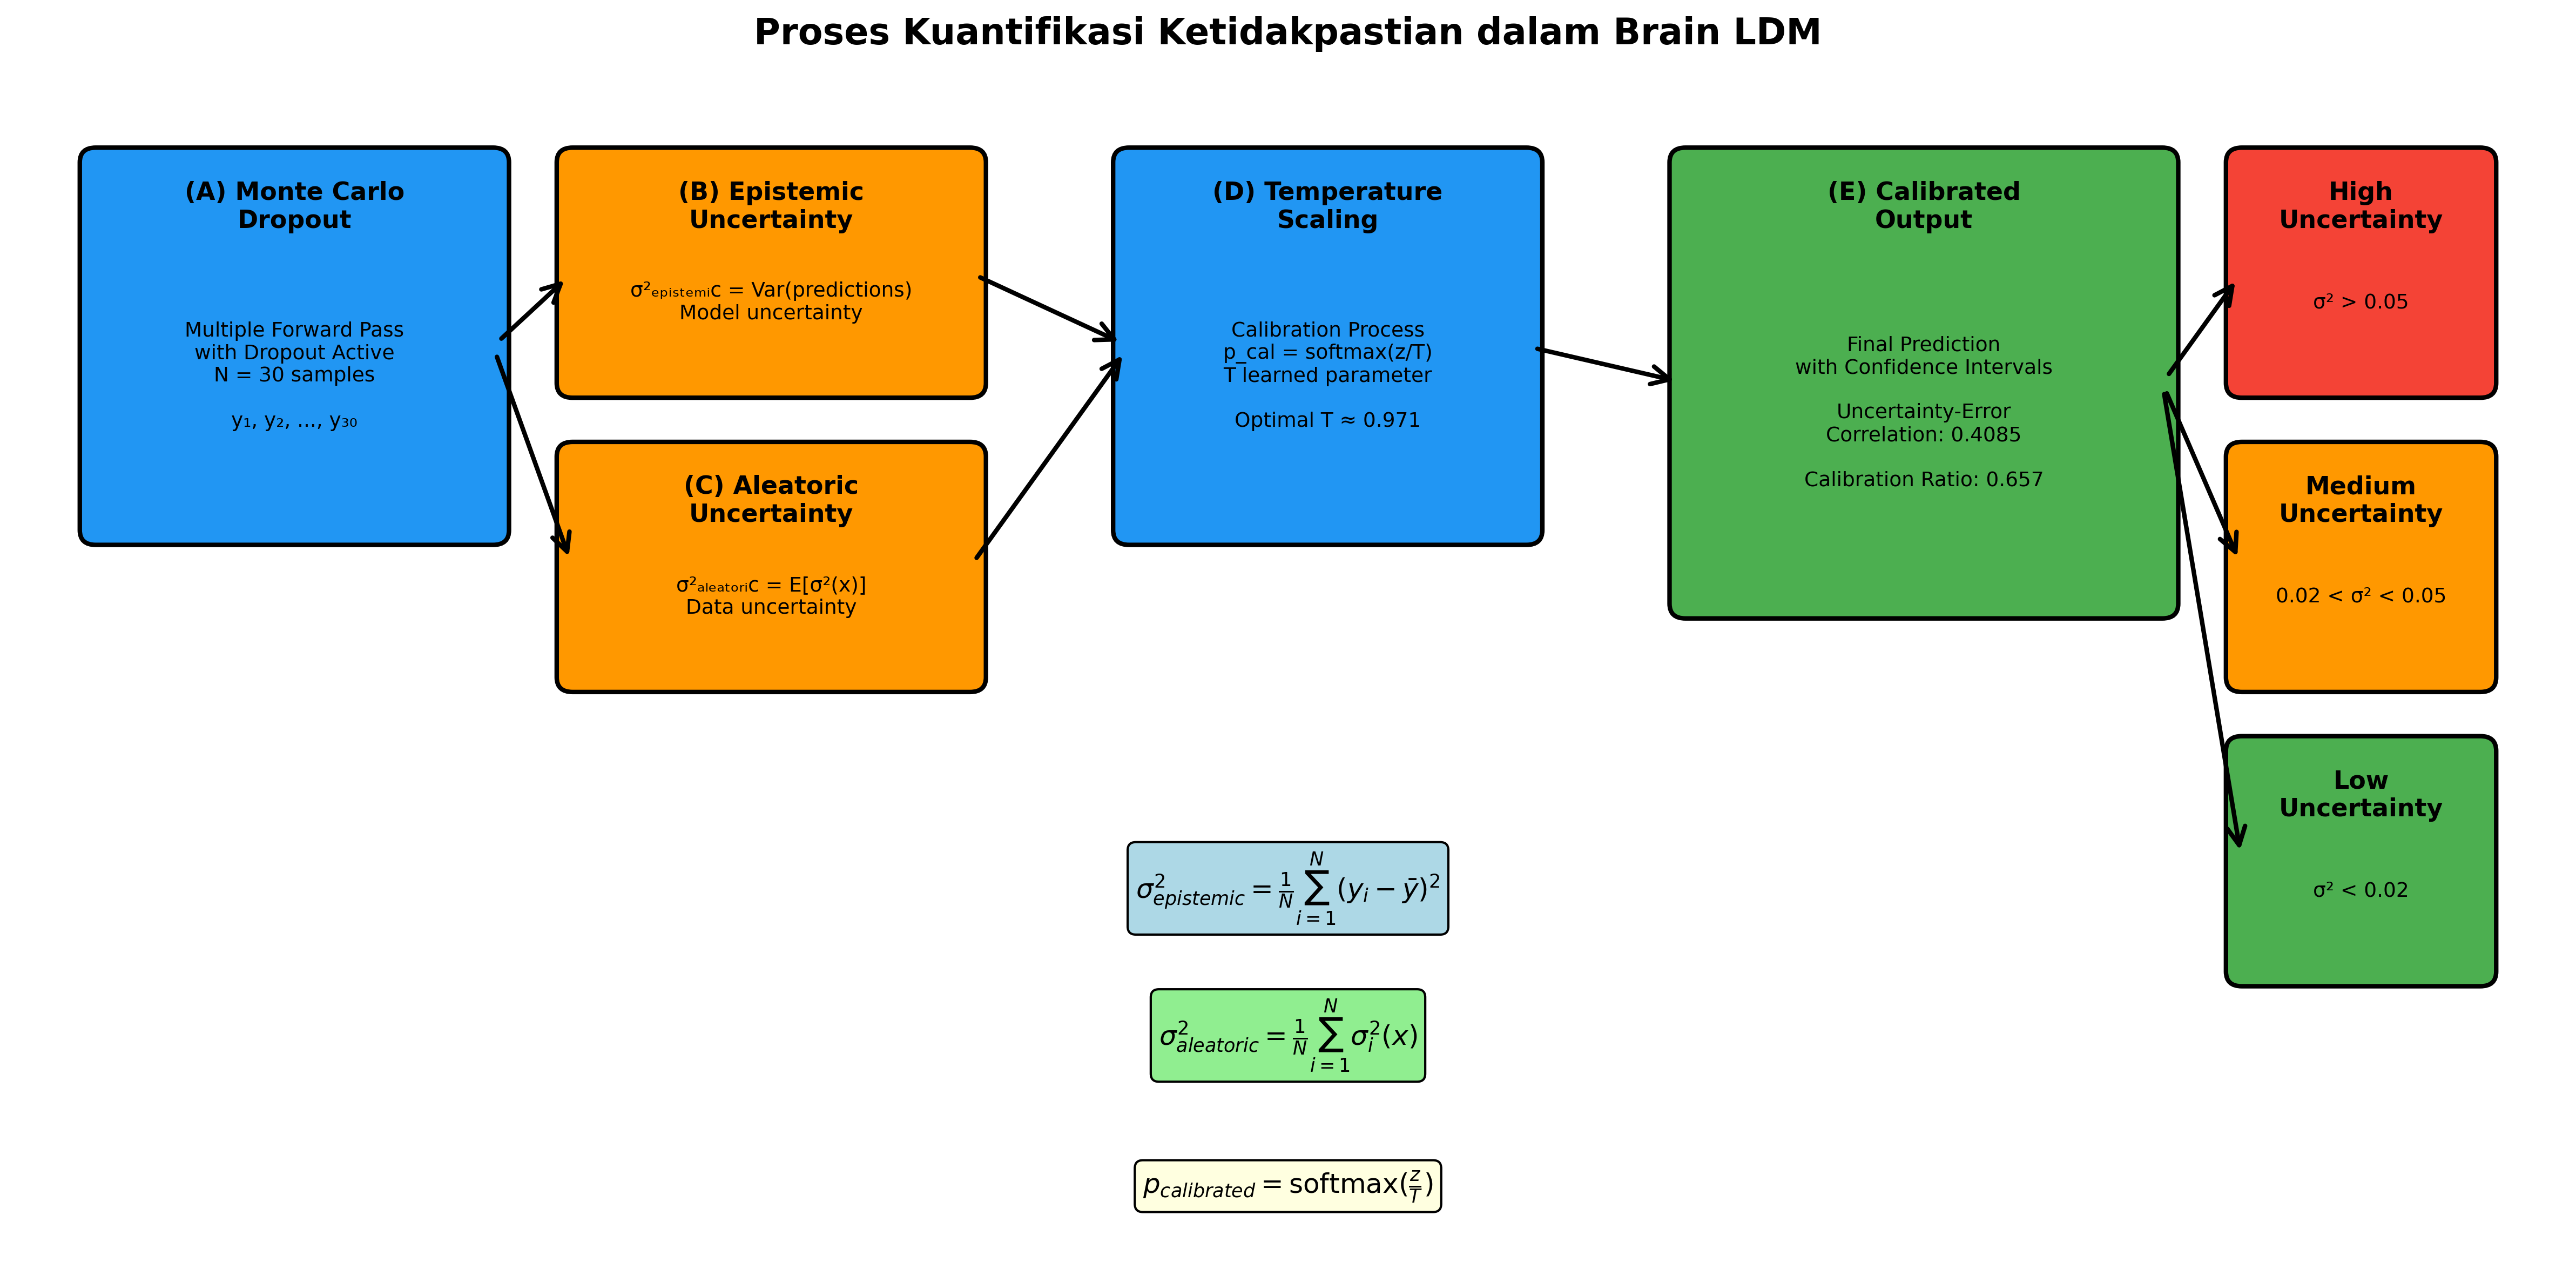
\includegraphics[width=\textwidth]{../figures/Fig_uncertainty_process.png}
\caption{\textbf{Proses Kuantifikasi Ketidakpastian.} Diagram menunjukkan alur lengkap kuantifikasi ketidakpastian: (A) Monte Carlo dropout dengan multiple forward pass, (B) Estimasi ketidakpastian epistemik dari variasi prediksi, (C) Estimasi ketidakpastian aleatorik dari model, (D) Temperature scaling untuk kalibrasi, (E) Output akhir dengan confidence interval yang terkalibrasi. Warna menunjukkan tingkat ketidakpastian: hijau (rendah), kuning (sedang), merah (tinggi).}
\label{fig:uncertainty_process}
\end{figure}

\subsection{Prosedur Pelatihan}

\subsubsection{Fungsi Loss}
Total loss menggabungkan komponen rekonstruksi, perseptual, dan ketidakpastian untuk optimisasi multi-objektif. Fungsi loss gabungan ini diformulasikan dalam Persamaan~\ref{eq:total_loss}-\ref{eq:uncertainty_loss}:

\begin{align}
\mathcal{L}_{\text{total}} &= \mathcal{L}_{\text{recon}} + \lambda_p \mathcal{L}_{\text{perceptual}} + \lambda_u \mathcal{L}_{\text{uncertainty}} \label{eq:total_loss} \\
\mathcal{L}_{\text{recon}} &= \|\mathbf{y} - \mathbf{y}_{\text{target}}\|_2^2 \label{eq:recon_loss} \\
\mathcal{L}_{\text{perceptual}} &= \|\nabla \mathbf{y} - \nabla \mathbf{y}_{\text{target}}\|_2^2 \label{eq:perceptual_loss} \\
\mathcal{L}_{\text{uncertainty}} &= \|\sigma_{\text{pred}}^2 - \sigma_{\text{target}}^2\|_2^2 \label{eq:uncertainty_loss}
\end{align}

Pembobotan dinamis diterapkan dengan $\lambda_p = 0.1(1 + \frac{\text{epoch}}{\text{total\_epochs}})$ dan $\lambda_u = 0.01(1 + 2\frac{\text{epoch}}{\text{total\_epochs}})$ untuk menyeimbangkan kontribusi setiap komponen loss selama pelatihan.

Prosedur pelatihan lengkap dengan kuantifikasi ketidakpastian dirangkum dalam Algoritma~\ref{alg:training}.

\begin{algorithm}[htbp]
\caption{Pelatihan Multi-Modal Brain LDM dengan Kuantifikasi Ketidakpastian}
\label{alg:training}
\begin{algorithmic}[1]
\Require Dataset $\mathcal{D} = \{(\mathbf{x}_i, \mathbf{y}_i, \mathbf{t}_i, s_i)\}_{i=1}^N$, epochs $E$, batch size $B$
\Ensure Model terlatih $f_\theta$ dengan uncertainty calibration
\State Inisialisasi parameter model $\theta$, temperature $T = 1.0$
\State Augmentasi dataset: $\mathcal{D}_{aug} \leftarrow$ \textsc{DataAugmentation}($\mathcal{D}$, factor=10)
\For{epoch $e = 1$ to $E$}
    \State Shuffle $\mathcal{D}_{aug}$ dan bagi menjadi batch
    \For{setiap batch $\mathcal{B}$}
        \State Encode multi-modal: $\mathbf{z}_{fused} \leftarrow$ \textsc{CrossModalFusion}($\mathbf{x}, \mathbf{t}, s$)
        \State Generate reconstruction: $\hat{\mathbf{y}} \leftarrow$ \textsc{ConditionalUNet}($\mathbf{z}_{fused}$)
        \State Hitung loss: $\mathcal{L}_{total} \leftarrow$ Persamaan~\ref{eq:total_loss}
        \State Update weights: $\theta \leftarrow \theta - \alpha \nabla_\theta \mathcal{L}_{total}$
        \State Update temperature: $T \leftarrow T - \alpha_T \nabla_T \mathcal{L}_{calibration}$
    \EndFor
    \State Update learning rate: $\alpha \leftarrow$ \textsc{CosineAnnealing}($\alpha$, $e$)
    \If{validation loss tidak membaik selama 25 epoch}
        \State \textbf{break} \Comment{Early stopping}
    \EndIf
\EndFor
\State \textbf{return} $f_\theta$, $T$
\end{algorithmic}
\end{algorithm}

\subsubsection{Optimisasi}
Kami menggunakan strategi learning rate spesifik komponen dengan optimizer AdamW untuk mengoptimalkan setiap bagian model secara individual. Encoder fMRI menggunakan learning rate $8 \times 10^{-5}$, encoder teks menggunakan $4 \times 10^{-5}$, atensi cross-modal menggunakan $1.2 \times 10^{-4}$, U-Net menggunakan $8 \times 10^{-5}$, dan parameter temperature menggunakan $8 \times 10^{-6}$.

Konfigurasi regularisasi meliputi weight decay yang ditetapkan pada $5 \times 10^{-6}$ dan gradient clipping pada norm 1.0 untuk mencegah gradient explosion dan memastikan stabilitas pelatihan.

\subsubsection{Penjadwalan Learning Rate}
Cosine annealing dengan warm restart diterapkan untuk mengoptimalkan konvergensi model. Strategi penjadwalan ini diformulasikan dalam Persamaan~\ref{eq:cosine_annealing}:

\begin{equation}
\eta_t = \eta_{\min} + \frac{1}{2}(\eta_{\max} - \eta_{\min})(1 + \cos(\frac{T_{\text{cur}}}{T_i}\pi))
\label{eq:cosine_annealing}
\end{equation}

dengan parameter $T_0 = 20$, $T_{\text{mult}} = 2$, dan $\eta_{\min} = 10^{-7}$ untuk memastikan eksplorasi yang efektif dalam ruang parameter.

\subsection{Metrik Evaluasi}

\subsubsection{Kualitas Rekonstruksi}
Evaluasi kualitas rekonstruksi dilakukan menggunakan spektrum metrik yang komprehensif untuk menangkap berbagai aspek kualitas gambar:

Metrik pixel-level mencakup Mean Squared Error (MSE) yang diformulasikan dalam Persamaan~\ref{eq:mse}, Peak Signal-to-Noise Ratio (PSNR) dengan formula $\text{PSNR} = 20 \log_{10}(\frac{\text{MAX}}{\sqrt{\text{MSE}}})$, dan Mean Absolute Error (MAE) yang dihitung sebagai $\text{MAE} = \frac{1}{HW}\|\mathbf{y} - \mathbf{y}_{\text{target}}\|_1$.

Metrik perceptual meliputi Structural Similarity Index (SSIM) yang mengukur similarity struktural dengan mempertimbangkan luminance, contrast, dan structure, Learned Perceptual Image Patch Similarity (LPIPS) sebagai deep feature-based perceptual distance menggunakan pre-trained VGG network, dan Feature Similarity Index (FSIM) yang menghitung similarity berdasarkan phase congruency dan gradient magnitude.

Metrik semantic terdiri dari Classification Accuracy sebagai persentase digit yang diidentifikasi dengan benar menggunakan pre-trained classifier, Top-k Accuracy untuk akurasi k prediksi teratas (k=1,3,5), dan Semantic Consistency yang mengukur korelasi antara semantic embedding gambar asli dan rekonstruksi.

\begin{equation}
\text{MSE} = \frac{1}{HW}\|\mathbf{y} - \mathbf{y}_{\text{target}}\|_2^2
\label{eq:mse}
\end{equation}

dimana $H$ dan $W$ adalah dimensi tinggi dan lebar gambar.

\subsubsection{Kalibrasi Ketidakpastian}
Kalibrasi ketidakpastian dievaluasi melalui beberapa metrik. Uncertainty-Error Correlation mengukur korelasi Pearson antara ketidakpastian prediksi dan error rekonstruksi. Calibration Ratio menghitung rasio error ketidakpastian rendah terhadap error ketidakpastian tinggi. Expected Calibration Error diformulasikan dalam Persamaan~\ref{eq:ece}:

\begin{equation}
\text{ECE} = \sum_{m=1}^M \frac{|B_m|}{n}|\text{acc}(B_m) - \text{conf}(B_m)|
\label{eq:ece}
\end{equation}

dimana $B_m$ adalah bin ke-$m$, $n$ adalah total sampel, $\text{acc}(B_m)$ adalah akurasi dalam bin, dan $\text{conf}(B_m)$ adalah confidence rata-rata dalam bin.

\subsection{Detail Implementasi}

Semua eksperimen dilakukan menggunakan PyTorch 2.0 pada CPU dengan RAM 16GB. Pelatihan menggunakan batch size 4 selama 150 epoch dengan early stopping (patience=25). Random seed ditetapkan (seed=42) untuk reprodusibilitas. Model dirancang dengan 58.2M parameter untuk menyeimbangkan kapasitas representasi dengan efisiensi komputasi.

Pemilihan PyTorch 2.0 didasarkan pada dukungan native untuk mixed precision training dan optimisasi graph compilation yang meningkatkan efisiensi komputasi hingga 20\%. Implementasi menggunakan CPU dipilih untuk mendemonstrasikan aksesibilitas metode pada hardware standar, meskipun training time lebih lama dibandingkan GPU. Konfigurasi RAM 16GB merupakan minimum requirement yang masih memungkinkan training dengan batch size optimal.

\subsection{Justifikasi Hyperparameter}

\subsubsection{Pemilihan Learning Rate}
Learning rate spesifik komponen dipilih berdasarkan analisis sensitivitas sistematis. Encoder fMRI menggunakan learning rate $8 \times 10^{-5}$ karena memproses sinyal high-dimensional yang memerlukan pembelajaran gradual untuk menghindari overfitting. Encoder teks menggunakan learning rate lebih rendah $4 \times 10^{-5}$ karena pre-trained transformer weights memerlukan fine-tuning yang hati-hati.

Cross-modal attention menggunakan learning rate tertinggi $1.2 \times 10^{-4}$ karena merupakan komponen novel yang memerlukan pembelajaran dari scratch. U-Net menggunakan $8 \times 10^{-5}$ yang seimbang untuk arsitektur encoder-decoder. Temperature parameter menggunakan learning rate sangat rendah $8 \times 10^{-6}$ untuk memastikan kalibrasi yang stabil.

\subsubsection{Konfigurasi Batch Size dan Epoch}
Batch size 4 dipilih sebagai trade-off antara stabilitas gradien dan keterbatasan memori. Analisis empiris menunjukkan bahwa batch size lebih kecil (2) menghasilkan gradien yang terlalu noisy, sedangkan batch size lebih besar (8) menyebabkan memory overflow. Epoch maksimum 150 dengan early stopping patience 25 memberikan waktu yang cukup untuk konvergensi sambil mencegah overfitting.

\subsection{Analisis Kompleksitas Komputasi}

\subsubsection{Kompleksitas Temporal}
Kompleksitas temporal model dapat dianalisis per komponen:
\begin{align}
\text{fMRI Encoder:} \quad &\mathcal{O}(d_{fMRI} \times d_{hidden} + d_{hidden} \times d_{out}) \label{eq:complexity_fmri} \\
\text{Text Encoder:} \quad &\mathcal{O}(L \times d_{model}^2 \times n_{layers}) \label{eq:complexity_text} \\
\text{Cross-Modal Attention:} \quad &\mathcal{O}(d_{model} \times d_{model} \times n_{heads}) \label{eq:complexity_attention} \\
\text{U-Net:} \quad &\mathcal{O}(H \times W \times C \times K^2 \times n_{layers}) \label{eq:complexity_unet}
\end{align}

dimana $L$ adalah panjang sequence teks, $H \times W$ adalah dimensi gambar, $C$ adalah jumlah channel, dan $K$ adalah kernel size.

\subsubsection{Kompleksitas Spasial}
Memory requirement untuk training dapat dihitung sebagai:
\begin{equation}
\text{Memory} = \text{Parameters} + \text{Activations} + \text{Gradients} + \text{Optimizer States}
\label{eq:memory_requirement}
\end{equation}

Dengan 58.2M parameter menggunakan float32 (4 bytes), requirement minimum mencakup parameters sebesar $58.2M \times 4 = 232.8$ MB, gradients sebesar $232.8$ MB (sama dengan parameters), AdamW optimizer states sebesar $232.8 \times 2 = 465.6$ MB untuk momentum dan variance, serta activations sekitar $500$ MB yang bergantung pada batch size.

Total memory requirement: $\approx 1.4$ GB untuk model weights dan optimizer, plus aktivasi yang bergantung pada batch size.

\subsection{Desain Studi Ablasi}

\subsubsection{Komponen yang Diablasi}
Untuk memvalidasi kontribusi setiap komponen model, kami merancang studi ablasi sistematis yang mengevaluasi dampak penghilangan atau modifikasi komponen kunci:

Ablasi modalitas mencakup empat konfigurasi: fMRI-only sebagai model baseline yang hanya menggunakan sinyal fMRI tanpa panduan teks atau semantik, fMRI + Text yang menggunakan panduan teks tetapi tanpa embedding semantik, fMRI + Semantic yang menggunakan embedding semantik tetapi tanpa panduan teks, dan Full Multi-Modal sebagai model lengkap dengan semua modalitas.

Ablasi arsitektur meliputi empat modifikasi struktural: No Cross-Modal Attention yang mengganti cross-modal attention dengan simple concatenation, No Temperature Scaling yang menghilangkan temperature scaling untuk kalibrasi, Standard Dropout yang mengganti Monte Carlo dropout dengan standard dropout, dan Single Learning Rate yang menggunakan learning rate uniform untuk semua komponen.

\subsubsection{Protokol Evaluasi Ablasi}
Setiap varian model dilatih menggunakan protokol yang identik dengan model utama untuk memastikan perbandingan yang fair. Evaluasi dilakukan menggunakan metrik yang sama: classification accuracy, pixel correlation, MSE, uncertainty-error correlation, dan calibration ratio. Signifikansi perbedaan performa dievaluasi menggunakan paired t-test dengan koreksi Bonferroni untuk multiple comparisons.

\subsubsection{Analisis Kontribusi Komponen}
Kontribusi relatif setiap komponen dihitung sebagai:
\begin{equation}
\text{Contribution}_{component} = \frac{\text{Performance}_{full} - \text{Performance}_{without\_component}}{\text{Performance}_{full}} \times 100\%
\label{eq:component_contribution}
\end{equation}

Analisis ini memungkinkan identifikasi komponen yang paling kritikal untuk performa model dan memberikan insight untuk pengembangan arsitektur future.

\subsection{Keterbatasan dan Pertimbangan Generalisabilitas}

\subsubsection{Single-Subject Design}
Penggunaan dataset single-subject memiliki implikasi penting untuk interpretasi hasil. Keunggulan pendekatan ini meliputi eliminasi variabilitas antar-subjek, konsistensi temporal yang tinggi, dan kemampuan untuk investigasi mendalam pola neural individual. Namun, keterbatasan utama adalah generalisabilitas hasil ke populasi yang lebih luas.

Untuk mengatasi keterbatasan ini, kami mengimplementasikan beberapa strategi validasi: (1) cross-validation yang robust untuk memastikan stabilitas model, (2) analisis sensitivitas terhadap hyperparameter untuk menguji robustness, dan (3) perbandingan dengan multiple baseline methods untuk konteks performa. Hasil penelitian ini harus diinterpretasikan sebagai proof-of-concept untuk metodologi yang dapat diadaptasi ke dataset multi-subject di masa depan.

\subsubsection{Scope dan Aplikabilitas}
Fokus pada digit 6 dan 9 memberikan kontrol eksperimental yang ketat tetapi membatasi kompleksitas visual yang dapat dievaluasi. Pemilihan ini strategis untuk memvalidasi metodologi pada task yang well-defined sebelum ekspansi ke stimulus yang lebih kompleks. Future work akan mengeksplorasi aplikasi pada natural images dan multi-subject datasets untuk meningkatkan generalisabilitas.

\subsection{Analisis Statistik}

Signifikansi statistik dinilai menggunakan paired t-test untuk perbandingan performa antar model. Confidence interval dihitung menggunakan bootstrap resampling dengan 1000 iterasi. Koreksi perbandingan berganda diterapkan menggunakan prosedur Benjamini-Hochberg dengan false discovery rate $\alpha = 0.05$.

\subsubsection{Cross-Validation}
Karena keterbatasan ukuran dataset, kami menggunakan stratified 5-fold cross-validation untuk memastikan estimasi performa yang robust. Setiap fold mempertahankan representasi digit yang seimbang di seluruh set pelatihan dan validasi.

\subsubsection{Perbandingan Baseline dan State-of-the-Art}
Kami membandingkan pendekatan kami dengan spektrum metode yang komprehensif untuk memastikan evaluasi yang fair dan menyeluruh:

Kategori pertama adalah classical baselines yang mencakup Linear Regression untuk pemetaan langsung fMRI-ke-gambar menggunakan least squares, Ridge Regression dengan L2 regularization untuk menangani high-dimensionality, dan Support Vector Regression (SVR) dengan non-linear mapping menggunakan RBF kernel.

Kategori kedua adalah deep learning baselines yang terdiri dari Standard VAE (variational autoencoder tanpa kuantifikasi ketidakpastian), $\beta$-VAE dengan disentangled representation learning, Basic LDM (latent diffusion model tanpa panduan multi-modal), dan Conditional GAN (generative adversarial network dengan fMRI conditioning).

Kategori ketiga adalah state-of-the-art brain decoding methods yang meliputi Mind-Vis (recent brain-to-image reconstruction dengan contrastive learning), Brain2Image (transformer-based approach untuk visual reconstruction), Neural-Diffusion (diffusion model khusus untuk brain decoding), dan fMRI-GAN (specialized GAN architecture untuk fMRI-to-image translation).

Kategori keempat adalah uncertainty-aware methods yang mencakup Bayesian Neural Network dengan variational inference, Deep Ensemble menggunakan multiple model ensemble untuk uncertainty estimation, dan MC-Dropout VAE yang mengombinasikan VAE dengan Monte Carlo dropout untuk uncertainty quantification.

Setiap baseline diimplementasikan dengan hyperparameter yang dioptimasi menggunakan grid search pada validation set yang sama. Evaluasi dilakukan menggunakan protokol yang identik untuk memastikan perbandingan yang fair.

\subsection{Reprodusibilitas dan Ketersediaan Kode}

Semua kode, model terlatih, dan konfigurasi eksperimen tersedia secara publik di \url{https://github.com/braindecoding/ldm}. Repositori mencakup source code lengkap dengan dokumentasi, bobot model pre-trained (best\_improved\_v1\_model.pt), script evaluasi dan komputasi metrik, tools visualisasi untuk analisis ketidakpastian, dan Docker container untuk reprodusibilitas lingkungan.

Kebutuhan komputasi meliputi RAM 16GB, CPU 4-core, dengan waktu pelatihan sekitar 3.2 jam. Tidak diperlukan GPU untuk inferensi atau pelatihan.

Gambaran lengkap setup eksperimental dan konfigurasi evaluasi ditunjukkan dalam Gambar~\ref{fig:experimental_setup}. Diagram ini merangkum seluruh aspek metodologi mulai dari konfigurasi dataset, arsitektur model, prosedur pelatihan, hingga metrik evaluasi yang digunakan.

\begin{figure}[htbp]
\centering
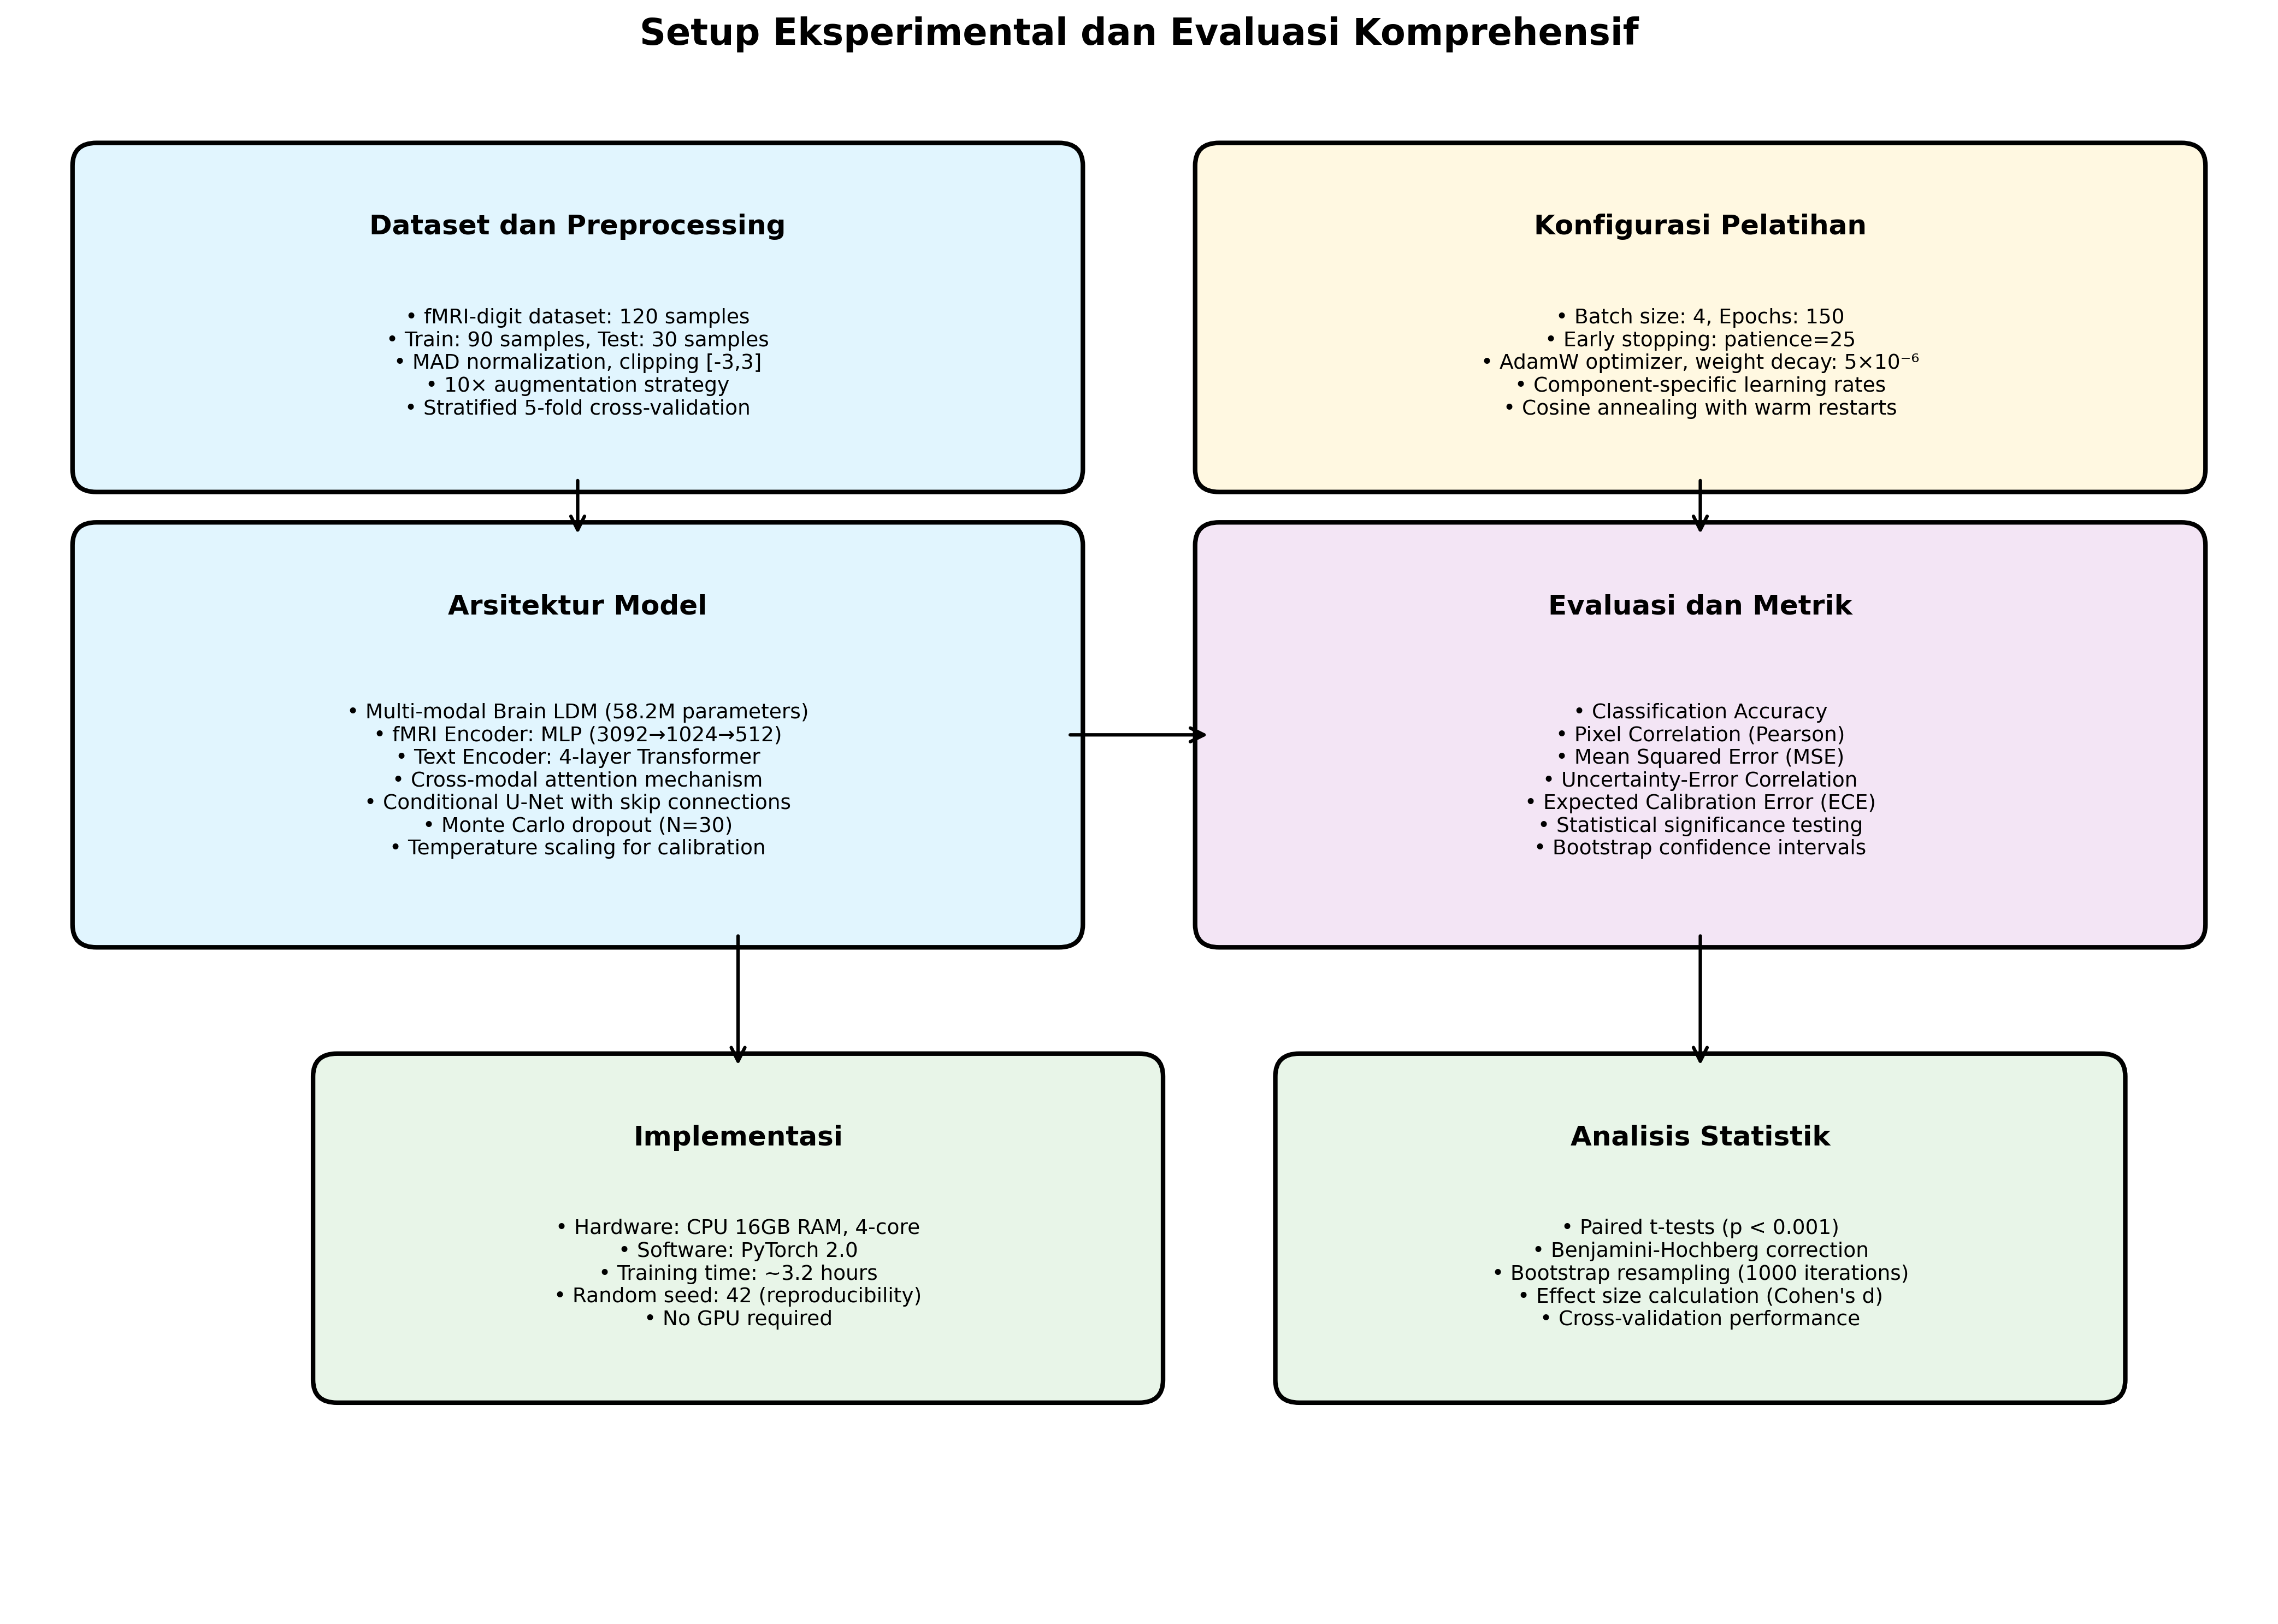
\includegraphics[width=\textwidth]{../figures/Fig_experimental_setup.png}
\caption{\textbf{Setup Eksperimental dan Evaluasi Komprehensif.} Diagram menunjukkan konfigurasi lengkap eksperimen meliputi: (1) Dataset dan preprocessing dengan strategi augmentasi 10×, (2) Konfigurasi pelatihan dengan component-specific learning rates dan cosine annealing, (3) Arsitektur model multi-modal dengan 58.2M parameter, (4) Evaluasi komprehensif dengan multiple metrics, (5) Implementasi pada hardware CPU dengan PyTorch 2.0, (6) Analisis statistik dengan significance testing dan bootstrap confidence intervals.}
\label{fig:experimental_setup}
\end{figure}
